\documentclass{article}

\usepackage[czech]{babel}
\usepackage[utf8]{inputenc}
\usepackage[T1]{fontenc}

\usepackage[left=2cm,text={17cm, 24cm},top=3cm, bottom=2cm]{geometry}

\usepackage{rotating}
\usepackage{graphicx} % vkládání obrázků
\usepackage{amsmath} % pokročilá sazba matematiky
% \usepackage{xcolor} % barevný text
\usepackage{siunitx} % SI jednotky
\usepackage{graphicx}
\usepackage{hyperref} % Clicable table of contents
\usepackage{color} % Color for table of contents
\usepackage{float}
\usepackage{lscape}
\usepackage{hyperref} 

\restylefloat{figure}

\hypersetup{
    colorlinks=true, %set true if you want colored links
    linktoc=all, %set to all if you want both sections and subsections linked
    linkcolor=black,  %choose some color if you want links to stand out
}

\graphicspath{ {./images} } % Include image folder

\begin{document}

% start first page
\clearpage
\begin{titlepage}
	\begin{center}
		\textsc{\LARGE Vysoké Učení Technické v Brně}\\[0.5cm]
		{\LARGE Fakulta informačních technologií }\\[4.0cm]

		\textsc{\LARGE IDS - Databázové systémy}\\[0.5cm]
		\textsc{\LARGE 2021/2022}\\[3.5cm]

		{\LARGE Projekt}\\[0.5cm]
    {\LARGE \textbf{Půjčovna hudebních nosičů}}\\
	\end{center}

	\vfill 

	\begin{flushleft} 
		\large
		Martin Douša (xdousa00)\\
    Zbyněk Pospíšil (xpospi0k)
		\hfill
		Brno, \today
	\end{flushleft}
\end{titlepage}
\thispagestyle{empty}

\newpage
\tableofcontents

\newpage
\listoffigures

\newpage
% end first page

\section {Zadání}

Navrhněte informační systém pro půjčovnu hudebních nosičů, který uchovává informace jak o zaměstnancích, tak o zákaznících. Ti si mohou jednotlivá alba vyhledávat přes katalog alb. Alba jsou v nabídce na různých nosičích a kvalitách (CD, DVD, kazeta, LP, minidisk, ...). Každé album obsahuje několik skladeb a může být v nabídce vícekrát i na různých typech nosičů. Jedna skladba může být obsažena ve více albech. Alba a skladby lze v katalogu vyhledávat pomocí názvu, interpreta, producenta, vydavatele, atd. Alba a skladby lze také vyhledávat podle jejich žánru, přičemž každá skladba i album mohou spadat do více žánrů (pop, rock, folk, country, disko, techno, metal, zaseknutá deska, ...). Zákazník si může najednou vypůjčit i více alb, pokud není album vráceno včas, systém zákazníkovi pošle upomínku. Podle doby překročení výpůjčky se vypočítá pokuta za dané album. U každé výpůjčky lze zpětně dohledat, který zaměstnanec ji zadal a kdo ji převzal.
\section{Model případů užití (Use Case Diagram)}

\begin{figure}[H] 
  \centering
  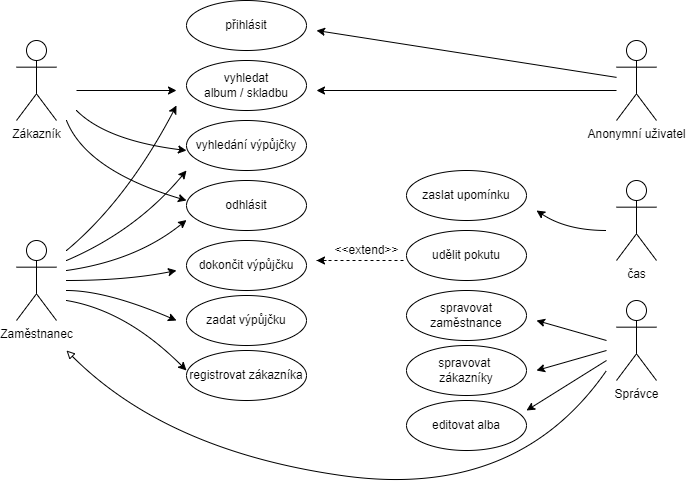
\includegraphics[scale=0.6,keepaspectratio]{usecase_diagram.png}
  \caption{Diagram připadů užití}
\end{figure}


\subsection{Popis}

\subsubsection{Anonymní uživatel}
Může vyhledat album nebo skladbu a může se přihlásit do systému.

\subsubsection{Zákazník}
Zákazník může vyhledat album nebo skladbu, vyhledat vlastní výpůjčky a podrobnosti o nich a odhlásit se ze systému.

\subsubsection{Zaměstnanec}
Zaměstnanec může vyhledat album nebo skladbu, vyhledat výpůjčky libovolného uživatele, zadat nebo dokončit výpůjčku, registrovat zákazníka a nebo se odhlásit.

\subsubsection{Správce (Zaměstnanec)}
Podle nastavených práv může správce spravovat zaměstnance, spravovat zákazníky a editovat alba.

\subsubsection{Čas}
Zasílá upomínky na vrácení výpůjčky

\section{ER Diagram}

\begin{figure}[H] 
  \centering
  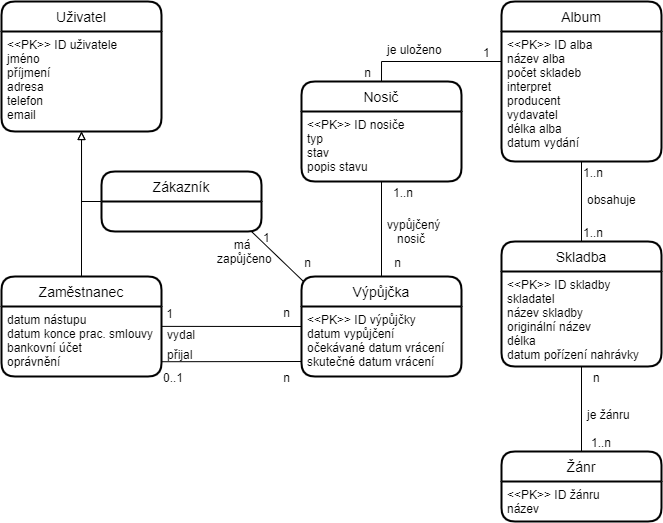
\includegraphics[scale=0.6,keepaspectratio]{er_diagram.png}
  \caption{ER Diagram}
\end{figure}


\subsection{Popis}

\subsubsection{Zákazník}
Zákazník má vypůjčeno \textbf{0 .. n} výpůjček.

\subsection{Album}
Album je uloženo na \textbf{0 .. n} nosičích (nemusí být naskladněno). \\
Album obsahuje \textbf{1 .. n} skladeb.

\subsection{Nosič}
Na nosiči je uloženo právě \textbf{1} album. \\
Nosič je by v \textbf{0 .. 1} výpůjčkách.

\subsection{Skladba}
Skladba je obsažena v \textbf{1 .. n} albech. \\
Skladba obsahuje \textbf{1 .. n} žánrů.

\subsection{Žánr}
Žánr je obsažen v \textbf{0 .. n} skladbách.

\subsection{Výpůjčka}
Výpůjčka obsahuje \textbf{1 .. n} nosičů. \\
Výpůjčce náleží \textbf{1} zákazník. \\
Výpůjčka byla vydána \textbf{1} zaměstnancem. \\
Výpůjčka byla přijata \textbf{0 .. 1} zaměstnancem.

\subsection{Zaměstnanec}
Zaměstnanec vydal \textbf{0 .. n} výpůjček. \\
Zaměstnanec přijal \textbf{0 .. n} výpůjček.

\end{document}